% Fix for: https://tex.stackexchange.com/a/315027/43228
\RequirePackage{luatex85}
\documentclass[border=10pt,17pt]{standalone}

\usepackage{cfr-lm}
\usepackage{pgf}
\usepackage{tikz}
\usetikzlibrary{arrows,shapes,snakes}
\usetikzlibrary{shapes.multipart}

\begin{document}

%% sans-serif fonts, large by default, and bold too
\sffamily
\sbweight
\bfseries
\large

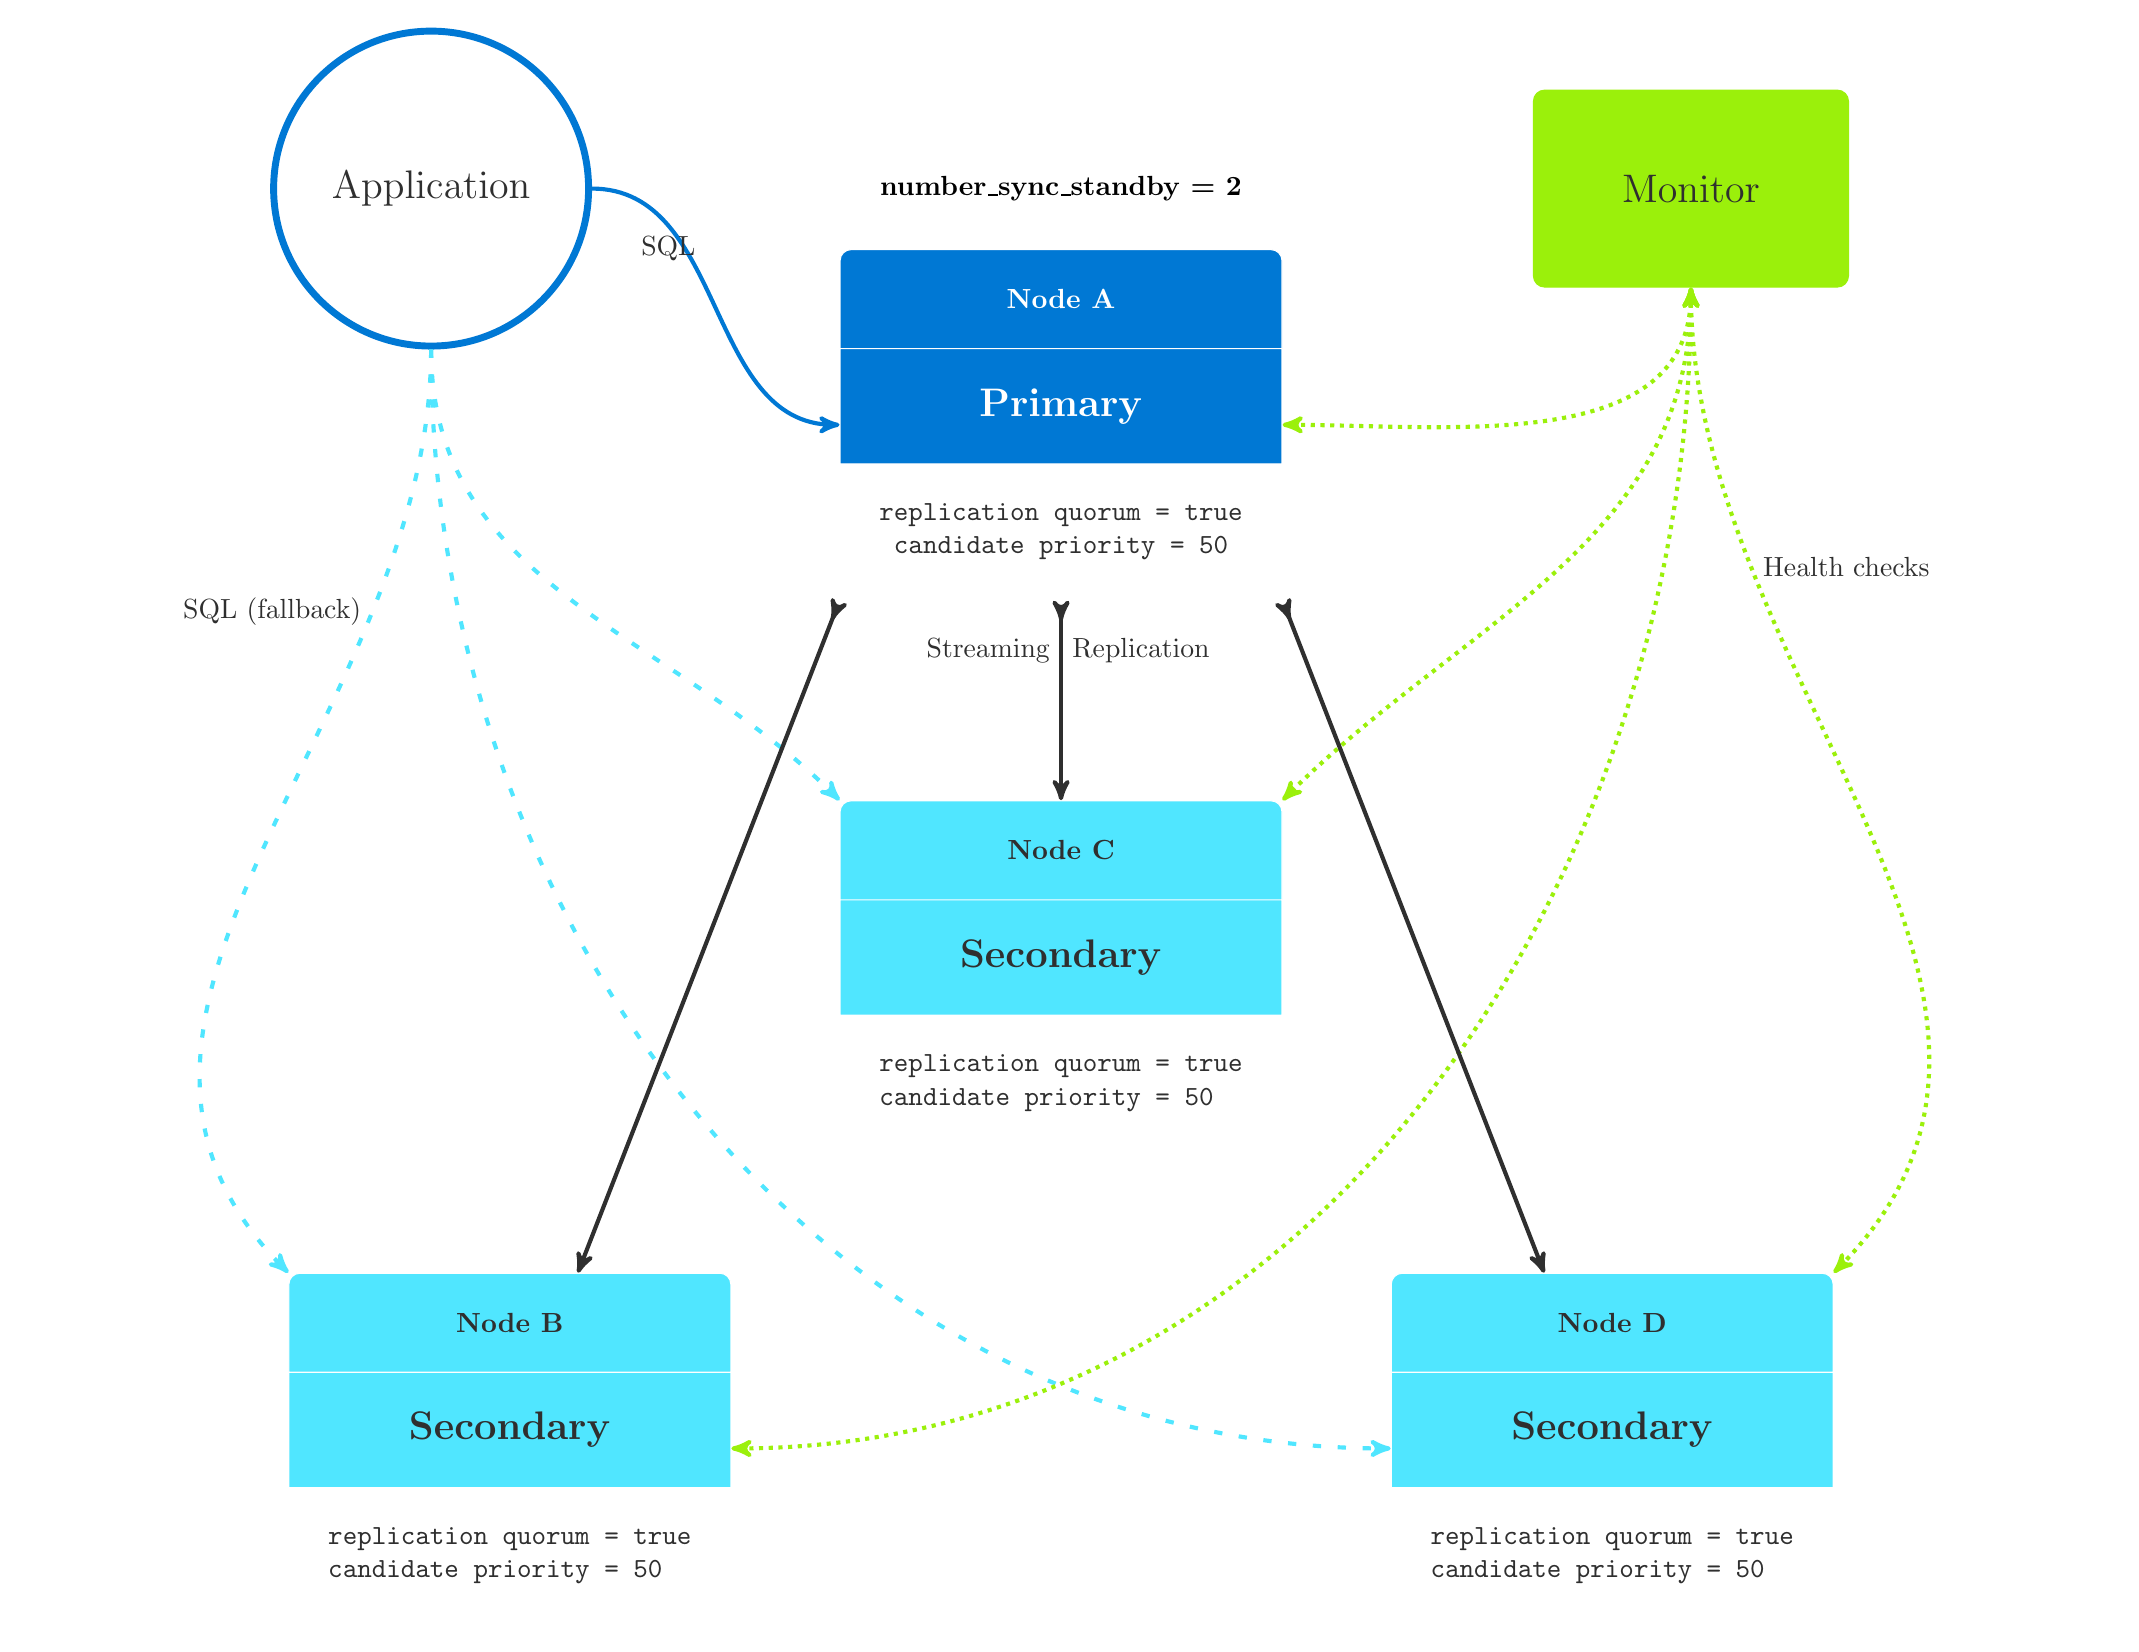
\begin{tikzpicture}[>=stealth',auto,rounded corners]

  \definecolor{pbox}{HTML}{0078D4} % MS blue
\definecolor{ptxt}{HTML}{FFFFFF} % white

\definecolor{sbox}{HTML}{50E6FF} % MS cyan
\definecolor{stxt}{HTML}{2F2F2F} % off-black

\definecolor{mbox}{HTML}{9BF00B} % MS light green
\definecolor{mtxt}{HTML}{2F2F2F} % off-black

\definecolor{apbox}{HTML}{0078D4} % MS blue
\definecolor{aptxt}{HTML}{2F2F2F} % off-black

\definecolor{async}{HTML}{EBEFF5} % very light grey

\tikzstyle{app}=[circle,thick,
	text=aptxt,draw=apbox,fill=white,
	line width=0.25em,minimum size=4cm]

\tikzstyle{node}=[rectangle,minimum height=2.5cm,minimum width=4cm]

\tikzstyle{mpnode}=[rectangle split,rectangle split parts=3,
	align=center,
	rectangle split part align={center, center, left},
	minimum height=2.5cm,minimum width=4cm,inner sep=0.5cm]

\tikzstyle{primary}=[mpnode,text=ptxt,draw=white,
  	rectangle split part fill={pbox,pbox,white}]

\tikzstyle{standby}=[mpnode,text=stxt,draw=white,
	rectangle split part fill={sbox,sbox,white}]

\tikzstyle{monitor}=[node,text=mtxt,draw=mbox,fill=mbox]

\tikzstyle{sql}=[->,color=pbox,text=stxt,line width=0.15em]
\tikzstyle{sqlf}=[->,color=sbox,text=stxt,line width=0.15em,loosely dashed]
\tikzstyle{sr}=[>->,color=stxt,text=stxt,line width=0.15em]
\tikzstyle{hc}=[<->,color=mbox,text=mtxt,line width=0.15em,dotted]


  %% \draw [help lines] (-10,0) grid (10,20);

  \node (flegend) at (0,18) {\textbf{\textt{number\_sync\_standby = 2}}} ;

  \node  (a)   at (0,15)   [primary]
         {\textbf{\normalsize Node A}
           \nodepart{second}
           \textbf{\Large Primary}
           \nodepart[text=stxt]{third}
           \texttt{replication quorum = true} \\
           \texttt{candidate priority = 50}
         };

  \node  (b)   at (-7,2)  [standby]
         {\textbf{\normalsize Node B}
           \nodepart{second}
           \textbf{\Large Secondary}
           \nodepart[align=left]{third}
           \texttt{replication quorum = true} \\
           \texttt{candidate priority = 50}
         };

  \node  (c)   at (0,8)   [standby]
         {\textbf{\normalsize Node C}
           \nodepart{second}
           \textbf{\Large Secondary}
           \nodepart[align=left]{third}
           \texttt{replication quorum = true} \\
           \texttt{candidate priority = 50}
         };

  \node  (d)   at (7,2)   [standby]
         {\textbf{\normalsize Node D}
           \nodepart{second}
           \textbf{\Large Secondary}
           \nodepart[align=left]{third}
           \texttt{replication quorum = true} \\
           \texttt{candidate priority = 50}
         };

  \node  (app) at (-8,18)  [app]        {\Large Application};
  \node  (m)   at (8,18)   [monitor]    {\Large Monitor};

  \path (app) edge [sql,out=0,in=180]  node[below,near start] {SQL} (a)
              edge [sqlf,out=-90,in=135]  node[left,near start] {SQL (fallback)} (b.north west)
              edge [sqlf,out=-90,in=135]  (c.north west)
              edge [sqlf,out=-90,in=180]  (d.west)

        (m)   edge [hc,out=-90,in=0] (a)
              edge [hc,out=-90,in=0] (b.east)
              edge [hc,out=-90,in=45] (c.north east)
              edge [hc,out=-90,in=45] node[right,near start] {Health checks} (d.north east)

        (a.south west) edge [sr] (b)
        (a) edge [sr] node[left,near start]  {Streaming} node[right,near start] {Replication} (c)
        (a.south east) edge [sr] (d);

\end{tikzpicture}

\end{document}
